\documentclass{article}
\usepackage{amsmath}
\usepackage{tikz}
\usetikzlibrary{shapes.geometric, arrows.meta, positioning, calc}

\begin{document}
	
	\section*{Volume of a Cone Using Integrals}
	
	Consider a right circular cone with radius $r$ and height $h$. We will calculate its volume using the method of integration. Let's take a cross-sectional disk with thickness $\Delta x$ at a distance $x$ from the apex of the cone.
	
	The radius of the disk, $R(x)$, is proportional to its distance $x$ from the apex. Therefore, we can write $R(x) = kx$, where $k$ is the proportionality constant. Since $R(h) = r$, we get $k = \frac{r}{h}$.
	
	Now, we can express the volume of the disk as $\Delta V = \pi R(x)^2 \Delta x = \pi k^2 x^2 \Delta x$. To find the volume of the entire cone, we integrate $\Delta V$ from $0$ to $h$.
	
	\begin{align*}
		V &= \int_{0}^{h} \pi k^2 x^2 dx \\
		&= \pi \left(\frac{r}{h}\right)^2 \int_{0}^{h} x^2 dx \\
		&= \pi \left(\frac{r}{h}\right)^2 \left[\frac{1}{3}x^3\right]_0^h \\
		&= \pi \left(\frac{r}{h}\right)^2 \left[\frac{1}{3}h^3 - 0\right] \\
		&= \frac{1}{3} \pi r^2 h
	\end{align*}
	
	Thus, the volume of the cone is given by:
	
	\begin{equation}
		V = \frac{1}{3} \pi r^2 h
	\end{equation}
	
	\begin{figure}[h]
		\centering
		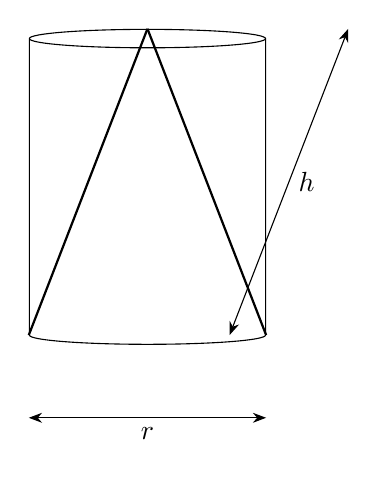
\begin{tikzpicture}[scale=1.5] % Adjust the scale factor here
			% Cone
			\node[draw, cylinder, shape border rotate=90, minimum height=4cm, minimum width=3cm] (cone) {};
			\draw[thick] (cone.before bottom) -- (cone.north);
			\draw[thick] (cone.after bottom) -- (cone.north);
			% Dimensions
			\draw[<->, >=Stealth] ($(cone.before bottom) - (0, 0.7)$) -- node[midway, below] {$r$} ($(cone.after bottom) - (0, 0.7)$);
			\draw[<->, >=Stealth] ($(cone.north) + (1.7, 0)$) -- node[midway, right] {$h$} ($(cone.after bottom) + (1.7, 0)$);
		\end{tikzpicture}
		\caption{A cone with radius $r$ and height $h$.}
	\end{figure}
	
\end{document}